\chapter{Preliminary}

As the target platform for this work is the graph database neo4J, we will mostly consider \textit{directed} graphs.
From the terminology we always refer \textit{arcs}, which is an directed edge.
In some cases we will refer to \textit{edges}, in these cases the direction doesn't play a role.

\section{Notation and Expressions}
We denote a graph $G(V, A)$ in case me mean an \textit{directed} graph, where $v$ is a vertex contained in the vertices $v \epsilon  V$ and $a$ is an arc $a \epsilon A$.
An arc is uniquely defined by to vertices $v_a$ and $v_b$ such that $v_a \neq v_b$, so there are no loops nor multi edges.
An arc has a weight function $w: A \rightarrow \mathbb{R}_{<0} $ that returns a positive integer.
\\
We use $A$ as the arc set and $a$ for a single directed arc.
$a \epsilon A$ can be replace with $e \epsilon E$ which refers to edges that are \textit{undirected}. 
\\
$G$ represents the input graph.
The index graph $G'(V', A')$ is the graph that will be used at contraction for initially building the CCH index structure.
A vertex $v$ in will never be really deleted.
Instead the rank property is set to mark this as an already contracted.
So $V \equiv V'$ but $A \subseteq A'$ there will be arcs add while building the CCH index.
$S = A' \setminus A$ is the shortcut set that is added throughout the contraction.
\\
We define the set of neighbors as $N(v)$, as vertices that are connected to $v$ with an arc. 
If only want the neighbors of higher rank we will use $N_\uparrow(v)$.
Analogously $N_\downarrow(v)$ defines the neighborhood of vertex $v$ that is of lower rank.
\\
We define the degree of an vertex $v$ as the number of neighbors this vertex has $|N(v)|$. 
The over all degree is the sum of a all upwards and downwards neighbors $|N(v)| = N_\uparrow(v) + N_\downarrow(v)$.
\\
The function on each graph $v : G \rightarrow \mathbb{N}_0$ that receives a positive integer and returns the vertex which has this rank assigned.
\\
$G^*(V^*, A^*)$ is the is the search graph while doing one a shortest path query.
Futhermore one query will have two search graphs.
$G^*_\uparrow$ representing the upwards search graph and the $G^*_\downarrow$.
\\
Finally there will be the edge set of edges that are written to the disk.
These will $\bigcirc A$ will be separated into to sets $\bigcirc A_\downarrow$ and $\bigcirc A_\uparrow $, too.

\section{Priority Queue}

One data structure that is heavily used in this paper is a priority queue.
This a very useful structure as it returns always the element with the lowest priority.
In dijkstra's algorithm for example, the priority is calculated on the path weight, so by retrieving an DijkstraState you will always get the smallest remaining.
The problem arises when it comes to updating an element of an priority queue that is already in the queue, because a priority queue can holt the same element multiple times and even with the different priorities.
The following explanation refers to the \cite[Java 17 reference]{JavaPrioQueue}, but priority queues are which based on a \cite[binary heap]{floyd1964algorithm} all have the same properties.
\\
One might ask why can't we simply remove the element that is already in the queue and then re-push it.
That is actually possible but slow, as the operations \textit{contains(element), and remove(element)} are running in linear time $\mathcal{O}(n) $.
Better would be to use \textit{offer(), poll(), remove() or add()} which run in logarithmic time $\mathcal{O}( \log (n))$.
One could think of just keeping a reference to the element and later on change the priority as needed.
But the queue will not be notified buy such a manipulation, and because the queue eagerly keeps the next element to dequeue at the top one will retrieve the wrong element.
So we have to cum up with something better.
If the priority of an element can only decrease, this usually doesn't cause a problem, because by retrieving an element you will definitely get the one with the lowest priority.
Therefore you can simply repush elements to the queue, as you will always get the real smallest possible.
To avoid processing an element twice you insert the elements into a set where you keep track of the already processed onces and if you retrieve a already seen one you simply poll again.
If the priority can decrease and increase and you simply push updated the elements to again, the problem is a bit more difficult as now you can possibly dequeue an element with the old priority which is lower as the current but not valid anymore.
We initialize a priority queue and a hash table which key is the element and the value is a integer a version number.
If we push an element to the queue we check whether the element is already in the control hash table, if not not we insert it together with the value $0$.
Then we wrap the element together with the $0$ and insert it into the queue.
If the element is already in the control hash table we increase the version number it has in the hash table by one, wrap this new version number together with the element and push it queue.
At pull we retrieve the element together with its current version number.
If the number is not equal to the one in the control hash table we simply pull again and check again until we find an element that is up to date. 
As a result we can keep $\mathcal{O}( \log (n))$ insert and run in constant time in hash table given there is a suitable hash function.

\section{Dijkstra} \label{sec:dijkstra}

\begin{figure}
    \centering
    \begin{frame}
    \frametitle{Dijkstra}
    Let's go from $v_2$ to $v_3$
    \vfill
    \begin{columns}
    \column{0.5\textwidth}
    \centering
    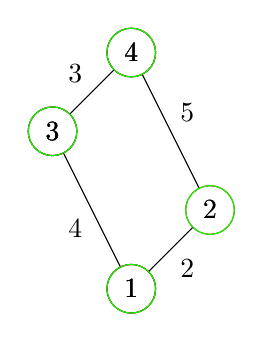
\begin{tikzpicture}[node distance={15mm}, main/.style = {draw, circle}]
        
        \onslide<1-2>{\node[main] (x3) at (0, 2) {$3$};}
        \onslide<3-4>{\node[main, draw=red] (x3) at (0, 2) {$3$};}
        \onslide<5->{\node[main, draw=green] (x3) at (0, 2) {$3$};}
        \onslide<1>{\node[main] (x4) at (1, 3) {$4$};}
        \onslide<2-3>{\node[main, draw=red] (x4) at (1, 3) {$4$};}
        \onslide<4->{\node[main, draw=green] (x4) at (1, 3) {$4$};}
        \onslide<1>{\node[main, draw=red] (x2) at (2, 1) {$2$};}
        \onslide<2->{\node[main, draw=green] (x2) at (2, 1) {$  2$};}
        \onslide<1>{\node[main] (x1) at (1, 0) {$1$};}
        \onslide<2>{\node[main, draw=red] (x1) at (1, 0) {$1$};}
        \onslide<3->{\node[main, draw=green] (x1) at (1, 0) {$1$};}
        
        \draw (x1) -- node[below right] {$2$}(x2);
        \draw (x1) -- node[below left] {$4$} (x3);
        \draw (x2) -- node[above right] {$5$} (x4);
        \draw (x3) -- node[above left] {$3$} (x4);

    \end{tikzpicture}
    \column{0.5\textwidth}
    \centering
    \begin{tabular}{c | c | c}
        \textbf{id} & \textbf{dist} & \textbf{settled}\\
        \hline 
        2 & 0  & \onslide<1>{false} \onslide<2->{true} \\ 
        \hline \pause
        1 & 2 & \onslide<2>{false} \onslide<3->{true}\\ 
        \hline
        4 &  5 & \onslide<2-3>{false} \onslide<4->{true} \\
        \hline \pause
        3 & 6 & \onslide<3-4>{false} \onslide<5->{true}\\ 
    \end{tabular}
\end{columns}
          
    

\end{frame}
    \caption{Dijkstra Class Diagram}
    \label{fig:dijkstra_class}
\end{figure}

Here, we want to explain dijkstra's algorithm as it crucial for the ch/cch search.
Additionally we want to decuple two thing that are usually done together.
The initialization of a dijkstra query and the iteration step, that expands vertices until the shortest path is found.
\\ 
Dijkstra finds the shortest path from a source vertex to a target vertex by always going the \textit{best} path.
Dijkstra starts with expanding the neighborhood of the source vertex and will move on to the vertex that has smallest total distance to the source vertex.
This is done until dijkstra is about to expand the target node next.
In the process of finding the target, dijkstra also finds the shortest path to every node it expands.
Therefore dijkstra cannot only be used to do \textit{one to one} shortest path queries, queries but also for \textit{one to many} and \textit{one to all} shortest path queries.
\\
Looking at figure \ref{fig:dijkstra_class} we initialize the query with a start id, a set of target ids and the graph on which we want to do the query.
At the construction process the query will take the start id, create an object of type \textit{DijkstraState} and push it to the \textit{queue}.
This priority queue is organized by the path weight of \textit{DijkstraState} such that it always returns the shortest path that is inside the queue.
\\
After the initialization, we can start expanding nodes using the \textit{expandNext()} method, which we provided in algorithm \ref{alg:disjkstra_algorithm}.
At first we pull the the next state from the queue.
Then we check whether the endVertex of the just retrieved state is in set of targets we are looking for or the set of goals is empty, mean we do a \textit{one to all} search.
If so we add the just found shortest path to the \textit{shortestPaths}.
Then we settle that state we know that we found the shortest path for the endVertex of this state.
Then we iterate over all arcs that are attached to this endVertex and therefore get its neighbors.
For each of this neighbors we check if we have to update it with a new state in the queue.
This is the case if either we haven't seen this vertex so far or the state in the queue is of higher weight as the one we just found.
\begin{frame}
    \frametitle{Dijkstra}
    Let's go from $v_2$ to $v_3$
    \vfill
    \begin{columns}
    \column{0.5\textwidth}
    \centering
    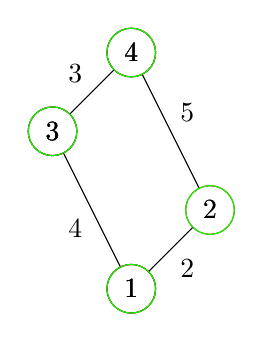
\begin{tikzpicture}[node distance={15mm}, main/.style = {draw, circle}]
        
        \onslide<1-2>{\node[main] (x3) at (0, 2) {$3$};}
        \onslide<3-4>{\node[main, draw=red] (x3) at (0, 2) {$3$};}
        \onslide<5->{\node[main, draw=green] (x3) at (0, 2) {$3$};}
        \onslide<1>{\node[main] (x4) at (1, 3) {$4$};}
        \onslide<2-3>{\node[main, draw=red] (x4) at (1, 3) {$4$};}
        \onslide<4->{\node[main, draw=green] (x4) at (1, 3) {$4$};}
        \onslide<1>{\node[main, draw=red] (x2) at (2, 1) {$2$};}
        \onslide<2->{\node[main, draw=green] (x2) at (2, 1) {$  2$};}
        \onslide<1>{\node[main] (x1) at (1, 0) {$1$};}
        \onslide<2>{\node[main, draw=red] (x1) at (1, 0) {$1$};}
        \onslide<3->{\node[main, draw=green] (x1) at (1, 0) {$1$};}
        
        \draw (x1) -- node[below right] {$2$}(x2);
        \draw (x1) -- node[below left] {$4$} (x3);
        \draw (x2) -- node[above right] {$5$} (x4);
        \draw (x3) -- node[above left] {$3$} (x4);

    \end{tikzpicture}
    \column{0.5\textwidth}
    \centering
    \begin{tabular}{c | c | c}
        \textbf{id} & \textbf{dist} & \textbf{settled}\\
        \hline 
        2 & 0  & \onslide<1>{false} \onslide<2->{true} \\ 
        \hline \pause
        1 & 2 & \onslide<2>{false} \onslide<3->{true}\\ 
        \hline
        4 &  5 & \onslide<2-3>{false} \onslide<4->{true} \\
        \hline \pause
        3 & 6 & \onslide<3-4>{false} \onslide<5->{true}\\ 
    \end{tabular}
\end{columns}
          
    

\end{frame}
\\
The \textit{expandNext()} procedure is what usually done in a while loop until the \textit{isComplete()} function returns \textit{true} and all requested shortest paths are found or all vertices have been expanded.
We provide this with the function \textit{getResult()} on such a dijkstra query object as you can see in figure \ref{fig:dijkstra_class}.
Being able to call the \textit{expandNext()} procedure from outside is a very powerful.
For example if we want to write a bidirectional dijkstra, we can create to two instances of the class \textit{Dijkstra} as stated in figure \ref{fig:dijkstra_class}.
One dijkstra is initialized only with outgoing $\text{Dijkstra(}s, [t,], \overrightarrow{G}(V, \overrightarrow{A}) \text{)}$ arcs the other only with incoming arcs $\text{Dijkstra(}t, [s], \overleftarrow{G}(V, \overleftarrow{A}) \text{)}$.
Now we can build our algorithm around that tells the bidirectional query when to stop or which side to expand next, but the essential thing here is we have reused the logic of the \textit{expandNext()} procedure and not written it again.

\section{Contraction Hierarchies}

Contraction Hierarchies \cite{Sanders} is a method that first arguments the graph with some additional edges that later on help Dijkstra's algorithm, such that it needs to expand fewer vertices.

\begin{figure}[H]
    \centering
    \begin{tikzpicture}[node distance={15mm}, main/.style = {draw, circle}]
    \node[main] (x3) at (0, 2) {$3$};
    \node[main] (x4) at (1, 3) {$4$};
    \node[main] (x2) at (2, 1) {$2$};
    \node[main] (x1) at (1, 0) {$1$};
    
    \draw (x1) -- node[below right] {$2$}(x2);
    \draw (x1) -- node[below left] {$1$} (x3);
    \draw (x2) -- node[above right] {$5$} (x4);
    \draw (x3) -- node[above left] {$1$} (x4);
    \draw[dashed] (x2) -- node[above, sloped] {$3$}  (x3);

    \draw[dashed]  (3,0) -- (3,3);


    \node[main] (x31) at (4, 2) {$3$};
    \node[main] (x21) at (6, 1) {$2$};
    \draw[ -Stealth, dashed] (x21) to node[above, sloped] {$3$}  (x31);

    \draw[dashed]  (7,0) -- (7,3);

    \node[main] (x32) at (8, 2) {$3$};
    \node[main] (x42) at (9, 3) {$4$};
    \node[main] (x22) at (10, 1) {$2$};

    \draw[-Stealth,] (x22) to node[above right] {$5$} (x42);
    \draw[-Stealth] (x42) to node[above left] {$1$} (x32);

\end{tikzpicture}
    \caption{Contraction Hierarchies simple example}
    \label{fig:ch_simple_example}
\end{figure}

Reading Figure \ref{fig:ch_simple_example} Contraction Hierarchies contracts, or deletes, vertices in a given order. 
The order we take is defined by the number you see inside the vertices, so CH contracts it in this order $v(1)$, $v(2)$, $v(3)$ and finally $v(4)$.
Only the solid lines are edges of the original graph.
The dashed line is a shortcut.
While contracting vertices it preserves the shortest path among the remaining vertices.
At first $v(1)$ is contracted and as $v(1)$ is on the shortest path between $v(2)$ and $v(3)$ a shortcut is inserted between them.
This is the only shortcut CH inserts in this small graph.
In a shortest path dijkstra will now be restricted to only expand edges from that are of higher rank.
To get all possible path CH does this one from the source vertex side expanding all outgoing edges and from the target side with all ingoing edges.
If we want to find the shortest path from $v(2)$ to $v(3)$, CH will expand all outgoing of $v(2)$ where it finds $v(3)$.
It also expands all ingoing of the target vertex $v(3)$ where it finds $v(4)$. 
Then both search side are merged at the meeting point which is $v(4)$ in this case.
As a result one get the path on the right in Figure \ref{fig:ch_simple_example}. 
The upwards search also find the a direct path from $v(2)$ to $v(3)$, which one can see in the middle of Figure \ref{fig:ch_simple_example}. 
Out of all these paths one take the shortest, which is also the shortest path in the original graph.
A shortcut does not only contain a weight information but also which vertex was contracted as it was inserted.
With this information the one can resolve the actual path in the graph.